\chapter{Experiments}

This chapter deals with discussing the experiment performed with different models to classify stereotypical social biases using the stereotypical dataset discussed in the previous section. Section \ref{task_overview} describes the basic overview of the classification task, with some insights into the data. Section \ref{experimental_setup}  discusses the basic setup for performing experiments. Section \ref{assessing_social_biases} describes the language models and baselines used, along with the training procedure. Finally, \ref{evaluation_metrics} describes about the evaluation metrics used when assessing the results.

\section{ Task overview}\label{task_overview}
The main goal of the thesis is to assess social stereotypes present in the text sequences using language models. The reasons for using language models which is based on transfer learning approach are as follows, firstly, when training a model using the classic supervised learning approach, where in, a model is trained on a dataset belonging to the source domain with training samples that demonstrate correct behavior and then tested on an identically distributed held out samples, the model tends to perform well \cite{ruder2019neural}. Moreover, these models require several hundred to thousands of samples to induce functions which generalize well \cite{radford2019language}. This approach might not suite for the task of assessing social stereotypes as the number of samples are relatively less. Transfer learning approach on the other hand is more preferable for the current setting where in the knowledge gained through training on the source domain/task is stored as representations (vectors) and applied to target domain or task \cite{ruder2019neural} rather than training from scratch as done in classic supervised learning approach. Transfer learning in the form of pretrained language models have become ubiquitous in natural language processing and contributed to state of the art on a wide range of tasks\cite{ruder2019transfer}. Due to the fact that the pre-trained language models have been trained on large amounts of real world data, the need for annotated data is reduced by 10x. Transfer learning using pre-trained language models have been shown to achieve similar performance compared to non-pretrained model with 10x fewer samples \cite{howard2018universal}. During this pre-training, they also capture the stereotypical biases present in the data \cite{nadeem2020stereoset}. This knowledge can thus be used for the target task of classifying stereotypical social biases. Considering these reasons, experiments have been performed on different pretrained language models. In order to evaluate the performance of language models and to answer the second research question of how far transfer learning can be used to detect stereotypes, baselines have been trained, which will be discussed in the corresponding section.

Considering the task of classification, several experiments using different combination of labels (stereotype, anti-stereotype, different bias types) and different classification tasks (binary, multi-class, multi label) have been performed to test the different perspectives of predictions. Finally, multi label classification was chosen with ethnicity, gender, profession, religion, stereotype, anti-stereotype, unrelated as labels. Considering the datasets stereoset and crowspair, as can be seen in the table \ref{tab:stereoset} and \ref{tab:Crowspair}, for each bias type there is a stereotypical as well as anti-stereotypical instance. Considering the perspective that stereotypes only have meaning to the extent they are socially shared \cite{macrae1996stereotypes}, anti-stereotype samples gives the perspective that the sample is a stereotype but not socially shared. Hence, considering anti-stereotype along with stereotype as a label gives the perspective whether a sample is socially share or not socially shared stereotype. To put it more clearly, stereotype samples are socially shared stereotypes, while anti-stereotypes are not socially shared stereotypes. Stereoset dataset also contain an unrelated instance per sample, this instance can be used as a sample which is neither socially shared (stereotype) nor not socially shared (anti-stereotype) but a totally unrelated sample. Hence, to the pre-processed dataset \ref{tab:Bias_type_stats_preprocessing}, anti-stereotypical samples from stereoset (combining context and anti\_stereotype instance ; see table \ref{tab:stereoset} for reference) and crowspair (sent\_less of crowspair; see table \ref{tab:Crowspair} for reference) are added. Stereoset Unrelated intersentence samples are added, excluding intrasentence unrelated. Considering the intrasentence stated in the table \ref{tab:stereoset}, the unrelated instance would be "girls tend to be more \textit{fish} than boys" which does not make any sense and thus are omitted. Data augmentation technique is used to generate unrelated synthetic samples using NLPaug \footnote{\url{https://github.com/makcedward/nlpaug}} library. The unrelated samples of intersentence were used as reference to generate synthetic samples by substituting certain number of words (word augmenter). contextual word embeddings of roberta-base model is used to substitute the original word in the reference sentence using similarity measure between original word and the word embeddings of the model. Hence, the final dataset statistics after adding anti-stereotypical samples and unrelated samples are as shown in the figure \ref{tab:data_final_stats}.

% Please add the following required packages to your document preamble:
% \usepackage{booktabs}
% \usepackage{graphicx}
\begin{table}[]
\centering
\scalebox{0.3}{
\resizebox{\columnwidth}{!}{%
\begin{tabular}{@{}lr@{}}
\toprule
Biat type             & No. of samples             \\ \midrule
Ethnicity             & 5226                       \\
Profession            & 3112                       \\
Gender                & 2024                       \\
Religion              & 1953                       \\\bottomrule
\addlinespace
Total                 & 16560 \\ \bottomrule
% \multicolumn{1}{l|}{Total} & \multicolumn{1}{|l}{16560} \\ \bottomrule
\end{tabular}%
}}
\caption{Data statistics after combining anti-stereotypical and unrelated samples}
\label{tab:data_final_stats}
\end{table}


% Please add the following required packages to your document preamble:
% \usepackage{booktabs}
% \usepackage{graphicx}
\begin{table}[]
\resizebox{\textwidth}{!}{%
\begin{tabular}{@{}llllllll@{}}
\toprule
Ethnicity & Gender & Profession & Religion & Anti-stereotype & Stereotype & Unrelated & Sentence                                                         \\ \midrule
1 & 0 & 0 & 0 & 0 & 1 & 0 & Many people live in Ethiopia. The people are very thin and good at distance running \\
1         & 0      & 0          & 0        & 1               & 0          & 0         & Many people live in Ethiopia. The people are fat and unatheletic \\
0         & 0      & 0          & 0        & 0               & 0          & 1         & I saw a cowboy                                                   \\ \bottomrule
\end{tabular}%
}
\caption{One hot encoded stereotypical dataset }
\label{tab:ohe_df}
\end{table}

As shown in the table \ref{tab:ohe_df}, the final dataset consists of one hot encoded vectors where for each sample of stereotype (socially shared) or anti-stereotype (not socially shared), a corresponding bias type i.e. either ethnicity, gender, profession or religion is also present. This categorization thus answers whether a sample is a socially shared stereotype or not along with the bias type or its a totally unrelated sample.
% \begin{itemize}
%     \item Why transfer learning based approach ?
%     \begin{itemize}
%         \item Less number of samples available due to the multidimensional nature of stereotypes, and collecting and validating stereotypes is not a straight forward task.  
%         \item Use of the real world knowledge of language model to help felicitate the inadequacy. 
%     \end{itemize}
%     \item Why classification ?
%     \item Final goal of assessing stereotypical social bias in arguments produced by args.me search engine
% \end{itemize}

% Steps: 
% \begin{enumerate}
%     \item Collecting stereotypical samples with respect to different domains such as race, gender, profession etc. are gathered from the available sources (CrowS-Pairs \cite{nangia2020crows}, Social bias frames \cite{sap2019social}, StereoSet \cite{nadeem2020stereoset} as seen so far).
%     \item Exploratory data analysis for some insights into the different types of biases (gender, race, profession, religion).
%     \item Stereotypical dataset target labels interpretation
%         \begin{itemize}
%             \item Different perspectives of classification labels used 
%             \item Anti-stereotypical samples introduced to get the perspective whether a text sequence is socially shared or not socially shared, as stereotypes can be interpreted as pictures in head.
%             \item  Including unrelated as a category in classification, why?
%         \end{itemize}
%     \item Categorization experiments
%     \begin{itemize}
%         \item Binary classification 
%         \item Multi-class classification 
%         \item Multi-label classification 
%         \item Why going with multi-label ?? When considering anti-stereotypical 
%     \end{itemize}
% \end{enumerate}
\section{Experimental setup}
\label{experimental_setup}
All the experiments including language models and baselines in this thesis are performed using Google Colaboratory \footnote{\url{https://colab.research.google.com/}}. For training language models, one NVIDIA Tesla T4 GPU provided by google Colaboratory is used. Baseline models have also been trained using google colab on 12GB RAM. For training language models mainly three libraries were used hugging face transformers \footnote{\url{https://huggingface.co/transformers/}}, Ktrain \footnote{\url{https://github.com/amaiya/ktrain}} and PyTorch lightening \footnote{\url{https://www.pytorchlightning.ai/}}. RayTune \footnote{\url{https://docs.ray.io/en/latest/tune/index.html}} was used to perform hyperparameter search for the language models. Keras \footnote{\url{https://keras.io/}} and scikit learn \footnote{\url{https://scikit-learn.org/stable/}} libraries were used to train baseline models.

\section{Assessing stereotypical social bias} \label{assessing_social_biases}
As discussed in the previous section, multi-label classification task was chosen to assess stereotypical social biases present in text sequences. Considering research question 1, four different pre-trained language models have been selected to experiment, namely BERT \cite{devlin2018bert}, RoBERTa, \cite{liu2019roberta}, XLNet \cite{yang2019xlnet} and GPT-2  \cite{radford2019language}. The reason for choosing these models for experimenting are, the authors of steroset \cite{nadeem2020stereoset} and crowspair \cite{nangia2020crows} have used their datasets to assess the stereotypes encoded in the these language models itself, thus uncovering the different types of biases encoded in different language models. This information could be useful when interpreting the results after training the fine-tuned language models. In order to answer the second question, baseline models have been trained to evaluate the use of transfer learning. Devlin\cite{devlin2018bert} states that there are two approaches for applying the language representation, namely, feature-based approach where the language representation are applied as features to initialize the model; fine-tuning approach where the model itself is fine-tuned and trained end-to-end. In the following subsections, first, fine-tuning based approach using language models are described with the training procedure. In the next subsection, feature based approach trained on machine learning models from scratch by using different pre-trained embedding models and selected features is discussed. 
\subsection{Fine-tuning based approach}
As discussed in the previous section, four language models were selected and fine-tuned to the downstream task of multi-label text classification using the stereotypical dataset. The training pipeline followed in the fine-tuning based approach can be briefly divided into four stages as shown in the figure \footnote{\url{https://www.flaticon.com/}} \ref{fig:fine-tuning based approach}. Firstly, in the data preprocessing, the labels of stereotypical dataset needs to be transformed into one-hot-encoded vectors for multi-label classification. In a multi-label classification setup, each sample belongs to several non-overlapping classes \cite{sokolova2009systematic}. Formally, multi label learning can be defined as a learn function \textit{h}:X \rightarrow 2$^y$ from multi label training set $D$ = $\{(x_i,y_i)| 1 \leq i\leq m\}$; where  $x_i \in X$ denotes d - dimensional instance space or feature vector and $y_i \in y$ denotes the  set of labels associated with $X_i$ \cite{zhang2013review}. The popular method when dealing with this problem is to create a binary classifier for each label \cite{ji2008extracting}, where a binary output, 1- for positive classes and 0 for the rest is assigned to each class. 
It is like having m binary classifiers for m labels. 
\pagebreak

\begin{figure}[]
    \centering
    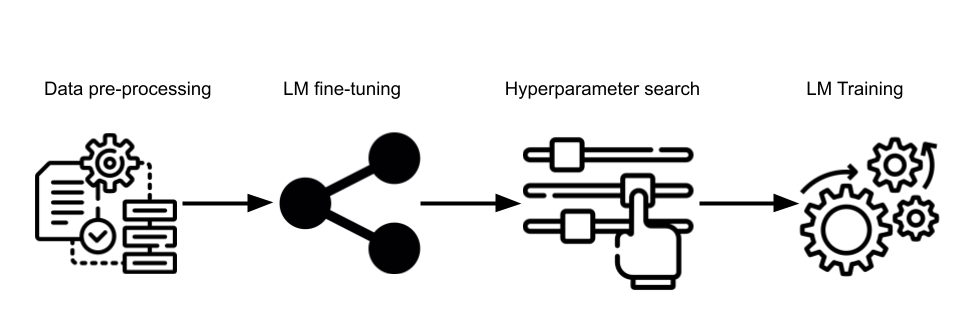
\includegraphics[width=0.7\textwidth]{thesis/figures/pipeline_changed.png}
    \caption{fine-tuning based approach pipeline}
    \label{fig:fine-tuning based approach}
\end{figure}

Hence, the labels of the stereotypical data are turned into one-hot encoded vectors as shown in the figure \ref{tab:ohe_df}. The one-hot encoded vectors are split into train, validation and test sets. Stratified train test splits  has been used to split the data into 70\% for training and 15\% for validation and test sets. Stratified sampling is helpful in preserving label/class proportion or composition \cite{merrillees2021stratified}. Next, the input data is to be processed according to the corresponding language model specifications, which is when the samples can be fed for training. This is done using hugging face auto tokenizer \footnote{\url{https://huggingface.co/transformers/model_doc/auto.html#transformers.AutoTokenizer}} class which consists of pretrained tokenizers to encode the input data according to the format the language model accepts. The basic steps done by auto tokenizer are as follows, split the input sentences into tokens, add special tokens corresponding to the language model ( Considering BERT language model \cite{devlin2018bert}, tokens $[CLS]$ is  added as first token to each input sentence to indicate the start of the sequence and $[SEP]$ added between two sentences as a separator for sentence pair tasks). Next, 'input\_ids', 'token\_type\_ids' and 'attention\_mask' corresponding to tokens of input sentence are generated. The input ids are based on vocabulary (look-up table) generated during the pre-training of the language model. Token type ids are used to indicate two pairs of sentences for sentence pair tasks and attention masks is used to indicate which tokens the model should pay attention to. When encoding batches of input sentences, the sentences should be padded to maximum length there in the batch and if the sentence length extends the maximum length the model can accept, they need to truncated. All these steps are handled by auto tokenizer of transformers. For our task, tokenizer.encode\_plus \footnote{\url{https://huggingface.co/transformers/internal/tokenization_utils.html#transformers.tokenization_utils_base.PreTrainedTokenizerBase.encode_plus}} is used to encode the text sequences with maximum length set to 50. This returns a dictionary of input\_ids, attention\_mask, labels. 

The next step is fine-tuning the language model to the target task, i.e. multi label classification. For this, hugging face transformers auto model \footnote{\url{https://huggingface.co/transformers/model_doc/auto.html#transformers.AutoModel}} has been used. This loads the corresponding language model with pretrained weights. For our downstream task of classification, a linear layer is added to the loaded model. Firstly, the outputs of the language model which represents the learned representations is to be selected/pooled as per the language model used. considering the running example BERT, the final hidden vector corresponding to $[CLS]$ token is used as input to the linear layer as prescribed by authors\cite{devlin2018bert}. Hence, a linear layer with size that of the last hidden unit and output size corresponding to the number of labels, In our case 7 is created. Considering BERT, the linear layer shape should be [768,7].  Finally, sigmoid activation function along with binary cross entropy loss function is used. Sigmoid activation function treats classes as non-overlapping mutually exclusive, hence used for multi-label classification and since multi label can be seen as several binary classifications, binary cross entropy loss function is used. This completes the fine-tuning step.

Coming to the next step, hyperparameter search of the fine-tuned language model is being done with the help of RayTune (a python library for experiment execution and hyperparameter tuning). Model hyperparameters can be defined as the parameters used to control the learning process which is set before training a model \cite{bergstra2012random} and the goal is to find optimal configuration parameters. The important steps for doing hyperparameter search is to define search space, search algorithm and a metric to evaluate the model with hyperparameters. The search space used is defined in the table \ref{tab:search_space}. Uniform method of ray tune samples a float value uniformly between the mentioned upper and lower limits. Choice method of ray tune samples a categorical value in the provided range\footnote{\url{https://docs.ray.io/en/latest/tune/api_docs/search_space.html}}. The search algorithm used is basicVarientGenerator \footnote{\url{https://docs.ray.io/en/releases-0.8.5/tune-searchalg.html#variant-generation-grid-search-random-search}} of ray which uses random search and grid search as algorithms. The objective metric is to reduce the validation loss. The models are run for 5 trials as shown in the table \ref{tab:search_trials} and the trial with minimum validation loss is chosen as the  the best hyperparameters for the model.  The hyperparameters obtained after running through the 5 trails are compiled in the following table \ref{tab:search_results}. Since, a common search space, search algorithm and same number of trials are used; this forms a common base for all the models for fair comparison.
% \begin{table}[]
% \centering
% \scalebox{0.5}{
% \resizebox{\textwidth}{!}{%
% \begin{tabular}{@{}llrrrr@{}}
% \toprule
%   & model\_name       & learning\_rate        & num\_train\_epochs & seed & per\_device\_train\_batch\_size \\ \midrule
% 0 & roberta-base      & 3.404460046972836e-05 & 5                  & 22   & 8                               \\
% 1 & xlnet-base-cased  & 2.49816047538945e-05  & 2                  & 15   & 32                              \\
% 2 & bert-base-uncased & 2.49816047538945e-05  & 2                  & 15   & 32                              \\
% 3 & gpt2              & 2.49816047538945e-05  & 2                  & 15   & 32                              \\ \bottomrule
% \end{tabular}%
% }}
% \caption{Hyperparameter search results for language models}
% \label{tab:search_results}
% \end{table}

% Please add the following required packages to your document preamble:
% \usepackage{booktabs}
% \usepackage{graphicx}
\begin{table}[]
\centering
\scalebox{0.7}{
\resizebox{\textwidth}{!}{%
\begin{tabular}{@{}ll@{}}
\toprule
Hyperparameter                  & Search space               \\ \midrule
learning\_rate                  & tune.uniform(1e-5,5e-5)    \\
num\_train\_epochs              & tune.choice({[}2,3,5{]})   \\
seed                            & tune.choice(range(1,41))   \\
per\_device\_train\_batch\_size & tune.choice({[}8,16,32{]}) \\ \bottomrule
\end{tabular}%
}}
\caption{Hyperparameter search space}
\label{tab:search_space}
\end{table}


% Please add the following required packages to your document preamble:
% \usepackage{booktabs}
% \usepackage{graphicx}
\begin{table}[]
\resizebox{\textwidth}{!}{%
\begin{tabular}{@{}rrrrr@{}}
\toprule
Trails & learning\_rate & num\_train\_epochs & per\_device\_train\_batch\_size & seed \\ \midrule
1           & 2.49816e-05    & 2                  & 32                              & 15   \\
2           & 4.11876e-05    & 2                  & 16                              & 39   \\
3           & 1.62398e-05    & 5                  & 8                               & 11   \\
4           & 3.40446r-05    & 5                  & 8                               & 22   \\
5           & 4.87964e-05    & 3                  & 16                              & 38   \\ \bottomrule
\end{tabular}%
}
\caption{Hyperparameter Search trails}
\label{tab:search_trials}
\end{table}

% Please add the following required packages to your document preamble:
% \usepackage{booktabs}
% \usepackage{graphicx}
\begin{table}[h!]
\resizebox{\textwidth}{!}{%
\begin{tabular}{@{}llrrrr@{}}
\toprule
  & model\_name       & learning\_rate        & num\_train\_epochs & seed & per\_device\_train\_batch\_size \\ \midrule
0 & roberta-base      & 3.404460046972836e-05 & 5                  & 22   & 8                               \\
1 & xlnet-base-cased  & 2.49816047538945e-05  & 2                  & 15   & 32                              \\
2 & bert-base-uncased & 2.49816047538945e-05  & 2                  & 15   & 32                              \\
3 & gpt2              & 2.49816047538945e-05  & 2                  & 15   & 32                              \\ \bottomrule
\end{tabular}%
}
\caption{Hyperparameter search results for language models}
\label{tab:search_results}
\end{table}

Finally, using these hyperparameters, the language models are trained. Here, the training of the fine-tuned model is done end-to-end as done by the authors of BERT \cite{devlin2018bert} while fine-tuning on different Natural language processing tasks. The procedure remains the same across all the language models used except for GPT-2 which is an autoregressive language model which would be explained in the next section.

\subsection{Brief description of language}
As described in the previous section four language models have been used and experimented with. Broadly, language models can be divided into autoencoding and autoregressive models \cite{yang2019xlnet}. Auto encoding models are models correspond to the encoder side of the original transformer \cite{vaswani2017attention} where the language models are pretrained by aiming to reconstruct the original data from the corrupted input data \cite{yang2019xlnet}. Autoregressive models on the other hand correspond to the decoder side of original transformers, where the model is trained on the classic language modelling task of estimating the probability distribution of a text corpus \cite{yang2019xlnet}. BERT and RoBERTa are purely auto encoding models, GPT-2 is a autoregressive model and xLNet is a generalized autoregressive model that builds on traditional autoregressive model. Some characteristic features of these language models  

\begin{itemize}
    \item Brief description of language models with main underlying features
    
    Language models :
    \begin{itemize}
        \item GPT-2 \cite{radford2019language}
        
            Features :
    \begin{itemize}
        \item Training data 
        \item Training procedure
        \begin{itemize}
            \item Pre-processing
            \item pre-training
        \end{itemize}
        \item encoded stereotypes (research from stereoset and crows pair)
    \end{itemize}
        \item BERT-base-uncased
        
            Features \cite{devlin2018bert}:
            \begin{itemize}
                \item Training data : BookCorpus (11,038 unpublished books) and English Wikipedia text articles  
                \item Training procedure
                \begin{itemize}
                    \item Pre-processing : Lowercased, tokenized using wordpiece and vocab of size 30,000
                \item pre-training 
                \end{itemize}
                \item encoded stereotypes (research from stereoset and crows pair)
    \end{itemize}
        \item RoBERTa \cite{liu2019roberta}
        
            Features :
            \begin{itemize}
                \item Training data 
                \item Training procedure
                \begin{itemize}
                    \item Pre-processing
                    \item pre-training
                \end{itemize}
                \item encoded stereotypes (research from stereoset and crows pair)
            \end{itemize}
        \item XLnet \cite{yang2019xlnet}
        
            Features :
            \begin{itemize}
                \item Training data 
                \item Training procedure
                \begin{itemize}
                    \item Pre-processing
                    \item pre-training
                \end{itemize}
                \item encoded stereotypes (research from stereo-set and crows pair)
            \end{itemize}
    \end{itemize}
    \item Why these language model?
    \item Training process
        \begin{itemize}
            \item Basic architecture of huggingface transformer models for sequence classification consists of 3 modules, namely, transformer module (pre-trained language model with weights), dropout (layer normalization), classifier (target specific layer). 
            \item  Doing hyper-parameter search using the RayTune \footnote{\url{https://docs.ray.io/en/master/tune/index.html}} a python library for experiment execution and hyper-parameter tuning with the described model with classification head attached. Model hyperparameters can be defined as the parameters used to control the learning process which is set before training a model. \cite{bergstra2012random}\textbf{add reference}.  The goal of hyper-parameter search/optimization is to find optimal parameters out of search space. The three important features of hyper-parameter search are defining search space, defining search algorithm which is used to select the hyper-parameters from the search space and finally a metric which is used to evaluate the model with the hyper-parameter. The search space used is defined below 
            \begin{itemize}
                \item Learning rate : tune.loguniform(1e-5, 5e-5)
                \item "num\_train\_epochs": tune.choice([2,3,5])
                \item "per\_device\_train\_batch\_size": tune.choice([8, 16, 32])
            \end{itemize}
            
        \begin{figure}[h]
            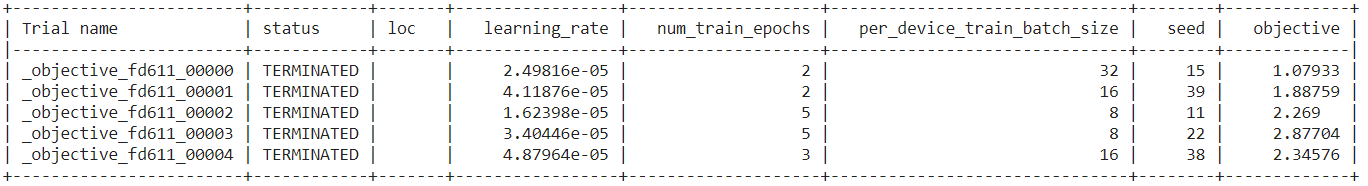
\includegraphics[width=12cm]{thesis/figures/hparameter.PNG}
            \centering
            \caption{Hyper-parameter search trails}
            \label{fig:The learning problem setup}
        \end{figure}
        
            \item Fine-tuning to target specific task (classification in our case) with target specific data (Multi-label dataset) by removing the language model head and replacing with 
            \begin{itemize}
                \item Linear layer with outputs corresponding to the number of labels 
                \item Adding corresponding activation function and loss function. As we are doing a multi label classification, we need to add a sigmoid activation function and binary cross entropy loss.
            \end{itemize}
        \item Training the fin-tuned model can be done by
        \begin{itemize}
            \item Training end - to - end wherein the entire fine-tuned model is trained and the loss is back-propagated to the entire network.
            \item Adaptive training where some layers of the initial layer of  pre-trained language model are freezed and the final layer of pre-trained model along with the attached classification head is trained. 
            \item Freezing the entire pre-trained model and only training the classification head attached. In this case only the  weights of the classification head are updated. 
        \end{itemize}
            
        \end{itemize}
\end{itemize}
\subsection{Feature based approach}

Questions:

\begin{enumerate}
    \item How does accuracy vary with non-contextual word embeddings (e.g. Glove, Word2Vec) to BERT word embedding?
    \item How does accuracy vary with baseline architecture (applying word embeddings to sentence and taking arithmetic average) to a fine-tuned BERT model ?
\end{enumerate}

    \begin{itemize}
        \item Lexicon - based approach : 
        \begin{itemize}
            \item Project into word embedding space and score each word based on its distance from woman, men ??
            \textbf{Refer }\cite{cryan2020detecting}
        \end{itemize}
        \item Brief description of  models and features
        \begin{itemize}
            \item SVM with selected lexicons + different features (toxicity, sentiment)
            \item Text-CNN with GLove,flair embedding
            \item Random embedding with GRU and LSTM 
        \end{itemize}
        \begin{itemize}
            \item Lexicons, POS and NER tags 
            \begin{itemize}
                \item Generalization : Plural nouns (NNS,NNPS), articles, article(the) + adjective(Refer to the whole group), determiner, quantifier (many,few, several...), frequency adverbs (Generic sentences - usually, typically, generally, sometimes, always)
                \item Subjectivity : strong subjectivity lexicon \cite{tangpersonalized}
                \item Syntactic cues : Syntactic negation (describing Stereotype-inconsistent )
            \end{itemize}
        \end{itemize}
        \item Why these model?
    \end{itemize}
    
\section{Evaluation metrics}\label{evaluation_metrics}

% \cite{tsoumakas2007multi}
\cite{zhang2013review}
    \begin{itemize}
        \item Label based Evaluation metrics
        \item Sample based evaluatoin metrics
        \item Evaluation metrics selected for multi-label classification 
        \item Hamming loss 
        \item AUC-ROC score 
        \item Precision, recall, f-measure with respect to different categories
    \end{itemize}
    
    
